% Created by tikzDevice version 0.12.6 on 2026-08-09 14:19:42
% !TEX encoding = UTF-8 Unicode
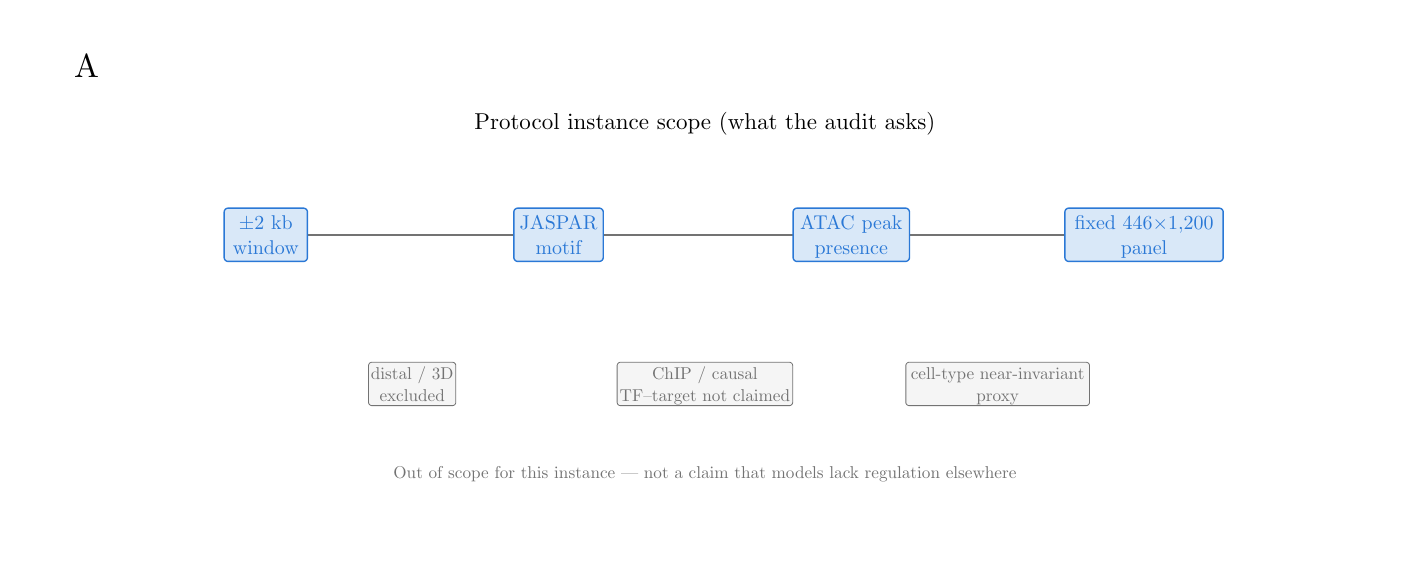
\begin{tikzpicture}[x=1pt,y=1pt]
\definecolor{fillColor}{RGB}{255,255,255}
\path[use as bounding box,fill=fillColor,fill opacity=0.00] (0,0) rectangle (491.44,187.90);
\begin{scope}
\path[clip] (  0.00,  0.00) rectangle (491.44,187.90);
\definecolor{drawColor}{RGB}{255,255,255}
\definecolor{fillColor}{RGB}{255,255,255}

\path[draw=drawColor,line width= 0.6pt,line join=round,line cap=round,fill=fillColor] (  0.00,  0.00) rectangle (491.44,187.90);
\end{scope}
\begin{scope}
\path[clip] (  4.00,  3.00) rectangle (485.44,183.90);

\path[] (  4.00,  3.00) rectangle (485.44,183.90);
\end{scope}
\begin{scope}
\path[clip] ( 12.00,  7.00) rectangle (477.44,177.90);
\definecolor{drawColor}{gray}{0.45}

\path[draw=drawColor,line width= 0.7pt,line join=round] ( 86.05,113.06) -- (403.39,113.06);
\definecolor{fillColor}{gray}{0.45}

\path[draw=drawColor,line width= 0.7pt,line join=round,fill=fillColor] (398.38,110.17) --
	(403.39,113.06) --
	(398.38,115.95) --
	cycle;
\definecolor{drawColor}{RGB}{42,120,214}
\definecolor{fillColor}{RGB}{217,232,248}

\path[draw=drawColor,line width= 0.5pt,line join=round,line cap=round,fill=fillColor] ( 72.45,103.44) --
	( 99.64,103.44) --
	( 99.59,103.44) --
	( 99.82,103.45) --
	(100.04,103.50) --
	(100.26,103.58) --
	(100.46,103.69) --
	(100.64,103.84) --
	(100.80,104.01) --
	(100.92,104.21) --
	(101.01,104.42) --
	(101.07,104.65) --
	(101.08,104.88) --
	(101.08,104.88) --
	(101.08,121.24) --
	(101.08,121.24) --
	(101.07,121.47) --
	(101.01,121.70) --
	(100.92,121.91) --
	(100.80,122.11) --
	(100.64,122.28) --
	(100.46,122.43) --
	(100.26,122.54) --
	(100.04,122.62) --
	( 99.82,122.67) --
	( 99.64,122.68) --
	( 72.45,122.68) --
	( 72.62,122.67) --
	( 72.39,122.68) --
	( 72.16,122.65) --
	( 71.94,122.59) --
	( 71.73,122.49) --
	( 71.54,122.36) --
	( 71.37,122.20) --
	( 71.23,122.01) --
	( 71.12,121.81) --
	( 71.05,121.59) --
	( 71.01,121.36) --
	( 71.01,121.24) --
	( 71.01,104.88) --
	( 71.01,105.00) --
	( 71.01,104.76) --
	( 71.05,104.53) --
	( 71.12,104.32) --
	( 71.23,104.11) --
	( 71.37,103.92) --
	( 71.54,103.76) --
	( 71.73,103.63) --
	( 71.94,103.53) --
	( 72.16,103.47) --
	( 72.39,103.44) --
	cycle;
\end{scope}
\begin{scope}
\path[clip] ( 12.00,  7.00) rectangle (477.44,177.90);
\definecolor{drawColor}{RGB}{42,120,214}

\node[text=drawColor,anchor=base,inner sep=0pt, outer sep=0pt, scale=  0.72] at ( 86.05,114.92) {$\pm$2 kb};

\node[text=drawColor,anchor=base,inner sep=0pt, outer sep=0pt, scale=  0.72] at ( 86.05,105.84) {window};
\end{scope}
\begin{scope}
\path[clip] ( 12.00,  7.00) rectangle (477.44,177.90);
\definecolor{drawColor}{RGB}{42,120,214}
\definecolor{fillColor}{RGB}{217,232,248}

\path[draw=drawColor,line width= 0.5pt,line join=round,line cap=round,fill=fillColor] (177.12,103.44) --
	(206.54,103.44) --
	(206.48,103.44) --
	(206.71,103.45) --
	(206.94,103.50) --
	(207.15,103.58) --
	(207.35,103.69) --
	(207.53,103.84) --
	(207.69,104.01) --
	(207.81,104.21) --
	(207.90,104.42) --
	(207.96,104.65) --
	(207.98,104.88) --
	(207.98,104.88) --
	(207.98,121.24) --
	(207.98,121.24) --
	(207.96,121.47) --
	(207.90,121.70) --
	(207.81,121.91) --
	(207.69,122.11) --
	(207.53,122.28) --
	(207.35,122.43) --
	(207.15,122.54) --
	(206.94,122.62) --
	(206.71,122.67) --
	(206.54,122.68) --
	(177.12,122.68) --
	(177.29,122.67) --
	(177.06,122.68) --
	(176.83,122.65) --
	(176.61,122.59) --
	(176.40,122.49) --
	(176.21,122.36) --
	(176.04,122.20) --
	(175.90,122.01) --
	(175.80,121.81) --
	(175.72,121.59) --
	(175.68,121.36) --
	(175.68,121.24) --
	(175.68,104.88) --
	(175.68,105.00) --
	(175.68,104.76) --
	(175.72,104.53) --
	(175.80,104.32) --
	(175.90,104.11) --
	(176.04,103.92) --
	(176.21,103.76) --
	(176.40,103.63) --
	(176.61,103.53) --
	(176.83,103.47) --
	(177.06,103.44) --
	cycle;
\end{scope}
\begin{scope}
\path[clip] ( 12.00,  7.00) rectangle (477.44,177.90);
\definecolor{drawColor}{RGB}{42,120,214}

\node[text=drawColor,anchor=base,inner sep=0pt, outer sep=0pt, scale=  0.72] at (191.83,114.92) {JASPAR};

\node[text=drawColor,anchor=base,inner sep=0pt, outer sep=0pt, scale=  0.72] at (191.83,105.84) {motif};
\end{scope}
\begin{scope}
\path[clip] ( 12.00,  7.00) rectangle (477.44,177.90);
\definecolor{drawColor}{RGB}{42,120,214}
\definecolor{fillColor}{RGB}{217,232,248}

\path[draw=drawColor,line width= 0.5pt,line join=round,line cap=round,fill=fillColor] (278.03,103.44) --
	(317.19,103.44) --
	(317.13,103.44) --
	(317.36,103.45) --
	(317.59,103.50) --
	(317.80,103.58) --
	(318.00,103.69) --
	(318.18,103.84) --
	(318.34,104.01) --
	(318.46,104.21) --
	(318.55,104.42) --
	(318.61,104.65) --
	(318.63,104.88) --
	(318.63,104.88) --
	(318.63,121.24) --
	(318.63,121.24) --
	(318.61,121.47) --
	(318.55,121.70) --
	(318.46,121.91) --
	(318.34,122.11) --
	(318.18,122.28) --
	(318.00,122.43) --
	(317.80,122.54) --
	(317.59,122.62) --
	(317.36,122.67) --
	(317.19,122.68) --
	(278.03,122.68) --
	(278.20,122.67) --
	(277.97,122.68) --
	(277.74,122.65) --
	(277.52,122.59) --
	(277.31,122.49) --
	(277.12,122.36) --
	(276.95,122.20) --
	(276.81,122.01) --
	(276.71,121.81) --
	(276.63,121.59) --
	(276.60,121.36) --
	(276.59,121.24) --
	(276.59,104.88) --
	(276.60,105.00) --
	(276.60,104.76) --
	(276.63,104.53) --
	(276.71,104.32) --
	(276.81,104.11) --
	(276.95,103.92) --
	(277.12,103.76) --
	(277.31,103.63) --
	(277.52,103.53) --
	(277.74,103.47) --
	(277.97,103.44) --
	cycle;
\end{scope}
\begin{scope}
\path[clip] ( 12.00,  7.00) rectangle (477.44,177.90);
\definecolor{drawColor}{RGB}{42,120,214}

\node[text=drawColor,anchor=base,inner sep=0pt, outer sep=0pt, scale=  0.72] at (297.61,114.92) {ATAC peak};

\node[text=drawColor,anchor=base,inner sep=0pt, outer sep=0pt, scale=  0.72] at (297.61,105.84) {presence};
\end{scope}
\begin{scope}
\path[clip] ( 12.00,  7.00) rectangle (477.44,177.90);
\definecolor{drawColor}{RGB}{42,120,214}
\definecolor{fillColor}{RGB}{217,232,248}

\path[draw=drawColor,line width= 0.5pt,line join=round,line cap=round,fill=fillColor] (376.23,103.44) --
	(430.55,103.44) --
	(430.49,103.44) --
	(430.72,103.45) --
	(430.95,103.50) --
	(431.16,103.58) --
	(431.36,103.69) --
	(431.54,103.84) --
	(431.70,104.01) --
	(431.82,104.21) --
	(431.91,104.42) --
	(431.97,104.65) --
	(431.98,104.88) --
	(431.98,104.88) --
	(431.98,121.24) --
	(431.98,121.24) --
	(431.97,121.47) --
	(431.91,121.70) --
	(431.82,121.91) --
	(431.70,122.11) --
	(431.54,122.28) --
	(431.36,122.43) --
	(431.16,122.54) --
	(430.95,122.62) --
	(430.72,122.67) --
	(430.55,122.68) --
	(376.23,122.68) --
	(376.41,122.67) --
	(376.18,122.68) --
	(375.95,122.65) --
	(375.72,122.59) --
	(375.51,122.49) --
	(375.32,122.36) --
	(375.16,122.20) --
	(375.02,122.01) --
	(374.91,121.81) --
	(374.84,121.59) --
	(374.80,121.36) --
	(374.79,121.24) --
	(374.79,104.88) --
	(374.80,105.00) --
	(374.80,104.76) --
	(374.84,104.53) --
	(374.91,104.32) --
	(375.02,104.11) --
	(375.16,103.92) --
	(375.32,103.76) --
	(375.51,103.63) --
	(375.72,103.53) --
	(375.95,103.47) --
	(376.18,103.44) --
	cycle;
\end{scope}
\begin{scope}
\path[clip] ( 12.00,  7.00) rectangle (477.44,177.90);
\definecolor{drawColor}{RGB}{42,120,214}

\node[text=drawColor,anchor=base,inner sep=0pt, outer sep=0pt, scale=  0.72] at (403.39,114.92) {fixed 446$\times$1{,}200};

\node[text=drawColor,anchor=base,inner sep=0pt, outer sep=0pt, scale=  0.72] at (403.39,105.84) {panel};
\end{scope}
\begin{scope}
\path[clip] ( 12.00,  7.00) rectangle (477.44,177.90);
\definecolor{drawColor}{gray}{0.45}
\definecolor{fillColor}{gray}{0.96}

\path[draw=drawColor,line width= 0.3pt,line join=round,line cap=round,fill=fillColor] (124.41, 51.32) --
	(153.46, 51.32) --
	(153.41, 51.32) --
	(153.61, 51.33) --
	(153.80, 51.37) --
	(153.99, 51.44) --
	(154.16, 51.54) --
	(154.32, 51.67) --
	(154.45, 51.82) --
	(154.55, 51.98) --
	(154.63, 52.17) --
	(154.68, 52.36) --
	(154.69, 52.56) --
	(154.69, 52.56) --
	(154.69, 65.76) --
	(154.69, 65.76) --
	(154.68, 65.96) --
	(154.63, 66.15) --
	(154.55, 66.33) --
	(154.45, 66.50) --
	(154.32, 66.65) --
	(154.16, 66.78) --
	(153.99, 66.87) --
	(153.80, 66.94) --
	(153.61, 66.98) --
	(153.46, 66.99) --
	(124.41, 66.99) --
	(124.56, 66.98) --
	(124.36, 66.99) --
	(124.17, 66.97) --
	(123.98, 66.91) --
	(123.80, 66.83) --
	(123.63, 66.72) --
	(123.49, 66.58) --
	(123.37, 66.42) --
	(123.28, 66.24) --
	(123.22, 66.05) --
	(123.18, 65.86) --
	(123.18, 65.76) --
	(123.18, 52.56) --
	(123.18, 52.66) --
	(123.18, 52.46) --
	(123.22, 52.26) --
	(123.28, 52.07) --
	(123.37, 51.90) --
	(123.49, 51.74) --
	(123.63, 51.60) --
	(123.80, 51.49) --
	(123.98, 51.40) --
	(124.17, 51.35) --
	(124.36, 51.32) --
	cycle;
\end{scope}
\begin{scope}
\path[clip] ( 12.00,  7.00) rectangle (477.44,177.90);
\definecolor{drawColor}{gray}{0.45}

\node[text=drawColor,anchor=base,inner sep=0pt, outer sep=0pt, scale=  0.62] at (138.94, 60.75) {distal / 3D};

\node[text=drawColor,anchor=base,inner sep=0pt, outer sep=0pt, scale=  0.62] at (138.94, 52.97) {excluded};
\end{scope}
\begin{scope}
\path[clip] ( 12.00,  7.00) rectangle (477.44,177.90);
\definecolor{drawColor}{gray}{0.45}
\definecolor{fillColor}{gray}{0.96}

\path[draw=drawColor,line width= 0.3pt,line join=round,line cap=round,fill=fillColor] (214.23, 51.32) --
	(275.20, 51.32) --
	(275.15, 51.32) --
	(275.35, 51.33) --
	(275.55, 51.37) --
	(275.73, 51.44) --
	(275.90, 51.54) --
	(276.06, 51.67) --
	(276.19, 51.82) --
	(276.30, 51.98) --
	(276.37, 52.17) --
	(276.42, 52.36) --
	(276.44, 52.56) --
	(276.44, 52.56) --
	(276.44, 65.76) --
	(276.44, 65.76) --
	(276.42, 65.96) --
	(276.37, 66.15) --
	(276.30, 66.33) --
	(276.19, 66.50) --
	(276.06, 66.65) --
	(275.90, 66.78) --
	(275.73, 66.87) --
	(275.55, 66.94) --
	(275.35, 66.98) --
	(275.20, 66.99) --
	(214.23, 66.99) --
	(214.38, 66.98) --
	(214.18, 66.99) --
	(213.99, 66.97) --
	(213.80, 66.91) --
	(213.62, 66.83) --
	(213.45, 66.72) --
	(213.31, 66.58) --
	(213.19, 66.42) --
	(213.10, 66.24) --
	(213.04, 66.05) --
	(213.00, 65.86) --
	(213.00, 65.76) --
	(213.00, 52.56) --
	(213.00, 52.66) --
	(213.00, 52.46) --
	(213.04, 52.26) --
	(213.10, 52.07) --
	(213.19, 51.90) --
	(213.31, 51.74) --
	(213.45, 51.60) --
	(213.62, 51.49) --
	(213.80, 51.40) --
	(213.99, 51.35) --
	(214.18, 51.32) --
	cycle;
\end{scope}
\begin{scope}
\path[clip] ( 12.00,  7.00) rectangle (477.44,177.90);
\definecolor{drawColor}{gray}{0.45}

\node[text=drawColor,anchor=base,inner sep=0pt, outer sep=0pt, scale=  0.62] at (244.72, 60.75) {ChIP / causal};

\node[text=drawColor,anchor=base,inner sep=0pt, outer sep=0pt, scale=  0.62] at (244.72, 52.97) {TF--target not claimed};
\end{scope}
\begin{scope}
\path[clip] ( 12.00,  7.00) rectangle (477.44,177.90);
\definecolor{drawColor}{gray}{0.45}
\definecolor{fillColor}{gray}{0.96}

\path[draw=drawColor,line width= 0.3pt,line join=round,line cap=round,fill=fillColor] (318.55, 51.32) --
	(382.45, 51.32) --
	(382.40, 51.32) --
	(382.59, 51.33) --
	(382.79, 51.37) --
	(382.97, 51.44) --
	(383.15, 51.54) --
	(383.30, 51.67) --
	(383.43, 51.82) --
	(383.54, 51.98) --
	(383.62, 52.17) --
	(383.66, 52.36) --
	(383.68, 52.56) --
	(383.68, 52.56) --
	(383.68, 65.76) --
	(383.68, 65.76) --
	(383.66, 65.96) --
	(383.62, 66.15) --
	(383.54, 66.33) --
	(383.43, 66.50) --
	(383.30, 66.65) --
	(383.15, 66.78) --
	(382.97, 66.87) --
	(382.79, 66.94) --
	(382.59, 66.98) --
	(382.45, 66.99) --
	(318.55, 66.99) --
	(318.70, 66.98) --
	(318.50, 66.99) --
	(318.31, 66.97) --
	(318.12, 66.91) --
	(317.94, 66.83) --
	(317.77, 66.72) --
	(317.63, 66.58) --
	(317.51, 66.42) --
	(317.42, 66.24) --
	(317.35, 66.05) --
	(317.32, 65.86) --
	(317.32, 65.76) --
	(317.32, 52.56) --
	(317.32, 52.66) --
	(317.32, 52.46) --
	(317.35, 52.26) --
	(317.42, 52.07) --
	(317.51, 51.90) --
	(317.63, 51.74) --
	(317.77, 51.60) --
	(317.94, 51.49) --
	(318.12, 51.40) --
	(318.31, 51.35) --
	(318.50, 51.32) --
	cycle;
\end{scope}
\begin{scope}
\path[clip] ( 12.00,  7.00) rectangle (477.44,177.90);
\definecolor{drawColor}{gray}{0.45}

\node[text=drawColor,anchor=base,inner sep=0pt, outer sep=0pt, scale=  0.62] at (350.50, 60.75) {cell-type near-invariant};

\node[text=drawColor,anchor=base,inner sep=0pt, outer sep=0pt, scale=  0.62] at (350.50, 52.97) {proxy};
\end{scope}
\begin{scope}
\path[clip] ( 12.00,  7.00) rectangle (477.44,177.90);
\definecolor{drawColor}{RGB}{0,0,0}

\node[text=drawColor,anchor=base,inner sep=0pt, outer sep=0pt, scale=  0.83] at (244.72,151.22) {Protocol instance scope (what the audit asks)};
\definecolor{drawColor}{gray}{0.45}

\node[text=drawColor,anchor=base,inner sep=0pt, outer sep=0pt, scale=  0.62] at (244.72, 25.15) {Out of scope for this instance --- not a claim that models lack regulation elsewhere};
\end{scope}
\begin{scope}
\path[clip] (  0.00,  0.00) rectangle (491.44,187.90);
\definecolor{drawColor}{RGB}{0,0,0}

\node[text=drawColor,anchor=base,inner sep=0pt, outer sep=0pt, scale=  1.20] at ( 21.31,170.04) {A};
\end{scope}
\end{tikzpicture}
